% SPDX-License-Identifier: CC-BY-4.0
% Figure 3 - HeraldRT architecture as implemented in rtl/ (qm_top on Kasli 2.0).
% Solid blocks exist in the RTL; dashed grey blocks are proposals.
% Grid: columns x = 8.4 / 11.8 / 15.4 / 18.3, rows y = 3.4 (Path A), 1.7, -1.6, -3.4, -5.3.
\documentclass[tikz, border=0pt]{standalone}
% SPDX-License-Identifier: CC-BY-4.0
% styles.tex - shared typography, colours and TikZ styles for all HeraldRT figures.
%
% Conventions used in every figure
%   optical path        red, solid, 1.2pt, open arrow head
%   electrical event    blue, solid, 0.9pt (detector pulses, herald)
%   control output      green, dashed, 0.9pt (electronics -> actuators)
%   host / config       grey, dotted
%   implemented block   solid outline     proposed block   dashed grey outline
%   asynchronous domain light amber fill  synchronous domain light blue fill

\usepackage{fontspec}
\usepackage{unicode-math}
\setmainfont{FiraSans}[
  Extension = .otf, UprightFont = *-Book, BoldFont = *-SemiBold,
  ItalicFont = *-BookItalic, BoldItalicFont = *-SemiBoldItalic]
\setsansfont{FiraSans}[
  Extension = .otf, UprightFont = *-Book, BoldFont = *-SemiBold,
  ItalicFont = *-BookItalic, BoldItalicFont = *-SemiBoldItalic]
\setmathfont{FiraMath-Regular.otf}
\setmonofont{FiraMono}[Extension = .otf, UprightFont = *-Regular, BoldFont = *-Medium,
  Scale = 0.92]
\renewcommand{\familydefault}{\sfdefault}

\usepackage[detect-all]{siunitx}
\sisetup{range-phrase = --, range-units = single, per-mode = symbol}

\usepackage{tikz}
\usetikzlibrary{arrows.meta, positioning, calc, fit, backgrounds,
  decorations.pathmorphing, decorations.markings, shapes.geometric, shapes.misc}

% layer for domain shading: above the white page, below blocks and wires
\pgfdeclarelayer{board}
\pgfdeclarelayer{domains}
\pgfsetlayers{background, board, domains, main}

% reproducible PDF (no creation date / ID differences between builds)
\pdfvariable suppressoptionalinfo 1023

% ------------------------------------------------------------------ colours
\definecolor{ink}{HTML}{1B2631}
\definecolor{optical}{HTML}{B03A2E}
\definecolor{opticallight}{HTML}{F2D7D5}
\definecolor{pumpviolet}{HTML}{6C3483}
\definecolor{elec}{HTML}{1F4E79}
\definecolor{ctrl}{HTML}{1E7B4A}
\definecolor{host}{HTML}{6E7B85}
\definecolor{asyncfill}{HTML}{FDF2E3}
\definecolor{asyncline}{HTML}{C07A1E}
\definecolor{syncfill}{HTML}{EAF2FA}
\definecolor{syncline}{HTML}{4F7FAF}
\definecolor{boxfill}{HTML}{FFFFFF}
\definecolor{muted}{HTML}{8A949C}
\definecolor{lat}{HTML}{C0392B}

\colorlet{proposed}{muted}

% ------------------------------------------------------------------ styles
\tikzset{
  every picture/.style = {line join = round, line cap = round, font = \small,
    text = ink, >={Stealth[length=2.2mm, width=1.6mm]}},
  % white page so the SVG stays readable in GitHub's dark mode
  white page/.style = {show background rectangle,
    background rectangle/.style = {fill = white, draw = none},
    inner frame xsep = 4mm, inner frame ysep = 3.5mm},
  % blocks
  block/.style = {draw = ink, line width = 0.7pt, fill = boxfill, rounded corners = 1.5pt,
    align = center, inner sep = 4pt, minimum height = 9mm},
  smallblock/.style = {block, font = \footnotesize, minimum height = 7mm, inner sep = 3pt},
  proposedblock/.style = {block, draw = proposed, dash pattern = on 3pt off 2pt,
    text = proposed, fill = white},
  device/.style = {block, fill = black!3},
  domain async/.style = {draw = asyncline, fill = asyncfill, line width = 0.6pt,
    rounded corners = 3pt, inner sep = 3.5mm},
  domain sync/.style = {draw = syncline, fill = syncfill, line width = 0.6pt,
    rounded corners = 3pt, inner sep = 3.5mm},
  board/.style = {draw = ink!70, line width = 0.7pt, rounded corners = 4pt, inner sep = 4mm},
  domain label/.style = {font = \footnotesize\bfseries, align = left},
  note/.style = {font = \footnotesize, text = ink!80, align = center},
  tag/.style = {font = \scriptsize, text = ink!70},
  % signals
  optical/.style = {draw = optical, line width = 1.2pt, -{Stealth[length=2.6mm, width=2mm]}},
  optical nohead/.style = {draw = optical, line width = 1.2pt},
  pump light/.style = {draw = pumpviolet, line width = 1.2pt, -{Stealth[length=2.6mm, width=2mm]}},
  elec/.style = {draw = elec, line width = 0.9pt, ->},
  ctrl/.style = {draw = ctrl, line width = 0.9pt, dash pattern = on 3.5pt off 2pt, ->},
  hostlink/.style = {draw = host, line width = 0.8pt, dash pattern = on 1pt off 1.6pt, <->},
  latency/.style = {circle, fill = lat, text = white, font = \scriptsize\bfseries,
    inner sep = 0.6pt, minimum size = 3.9mm},
}

% value-class tags used in the timing figure
\newcommand{\clsP}{\textsuperscript{\textcolor{optical}{\bfseries P}}}
\newcommand{\clsD}{\textsuperscript{\textcolor{asyncline}{\bfseries D}}}
\newcommand{\clsC}{\textsuperscript{\textcolor{ctrl}{\bfseries C}}}
\newcommand{\clsA}{\textsuperscript{\textcolor{host}{\bfseries A}}}


\begin{document}
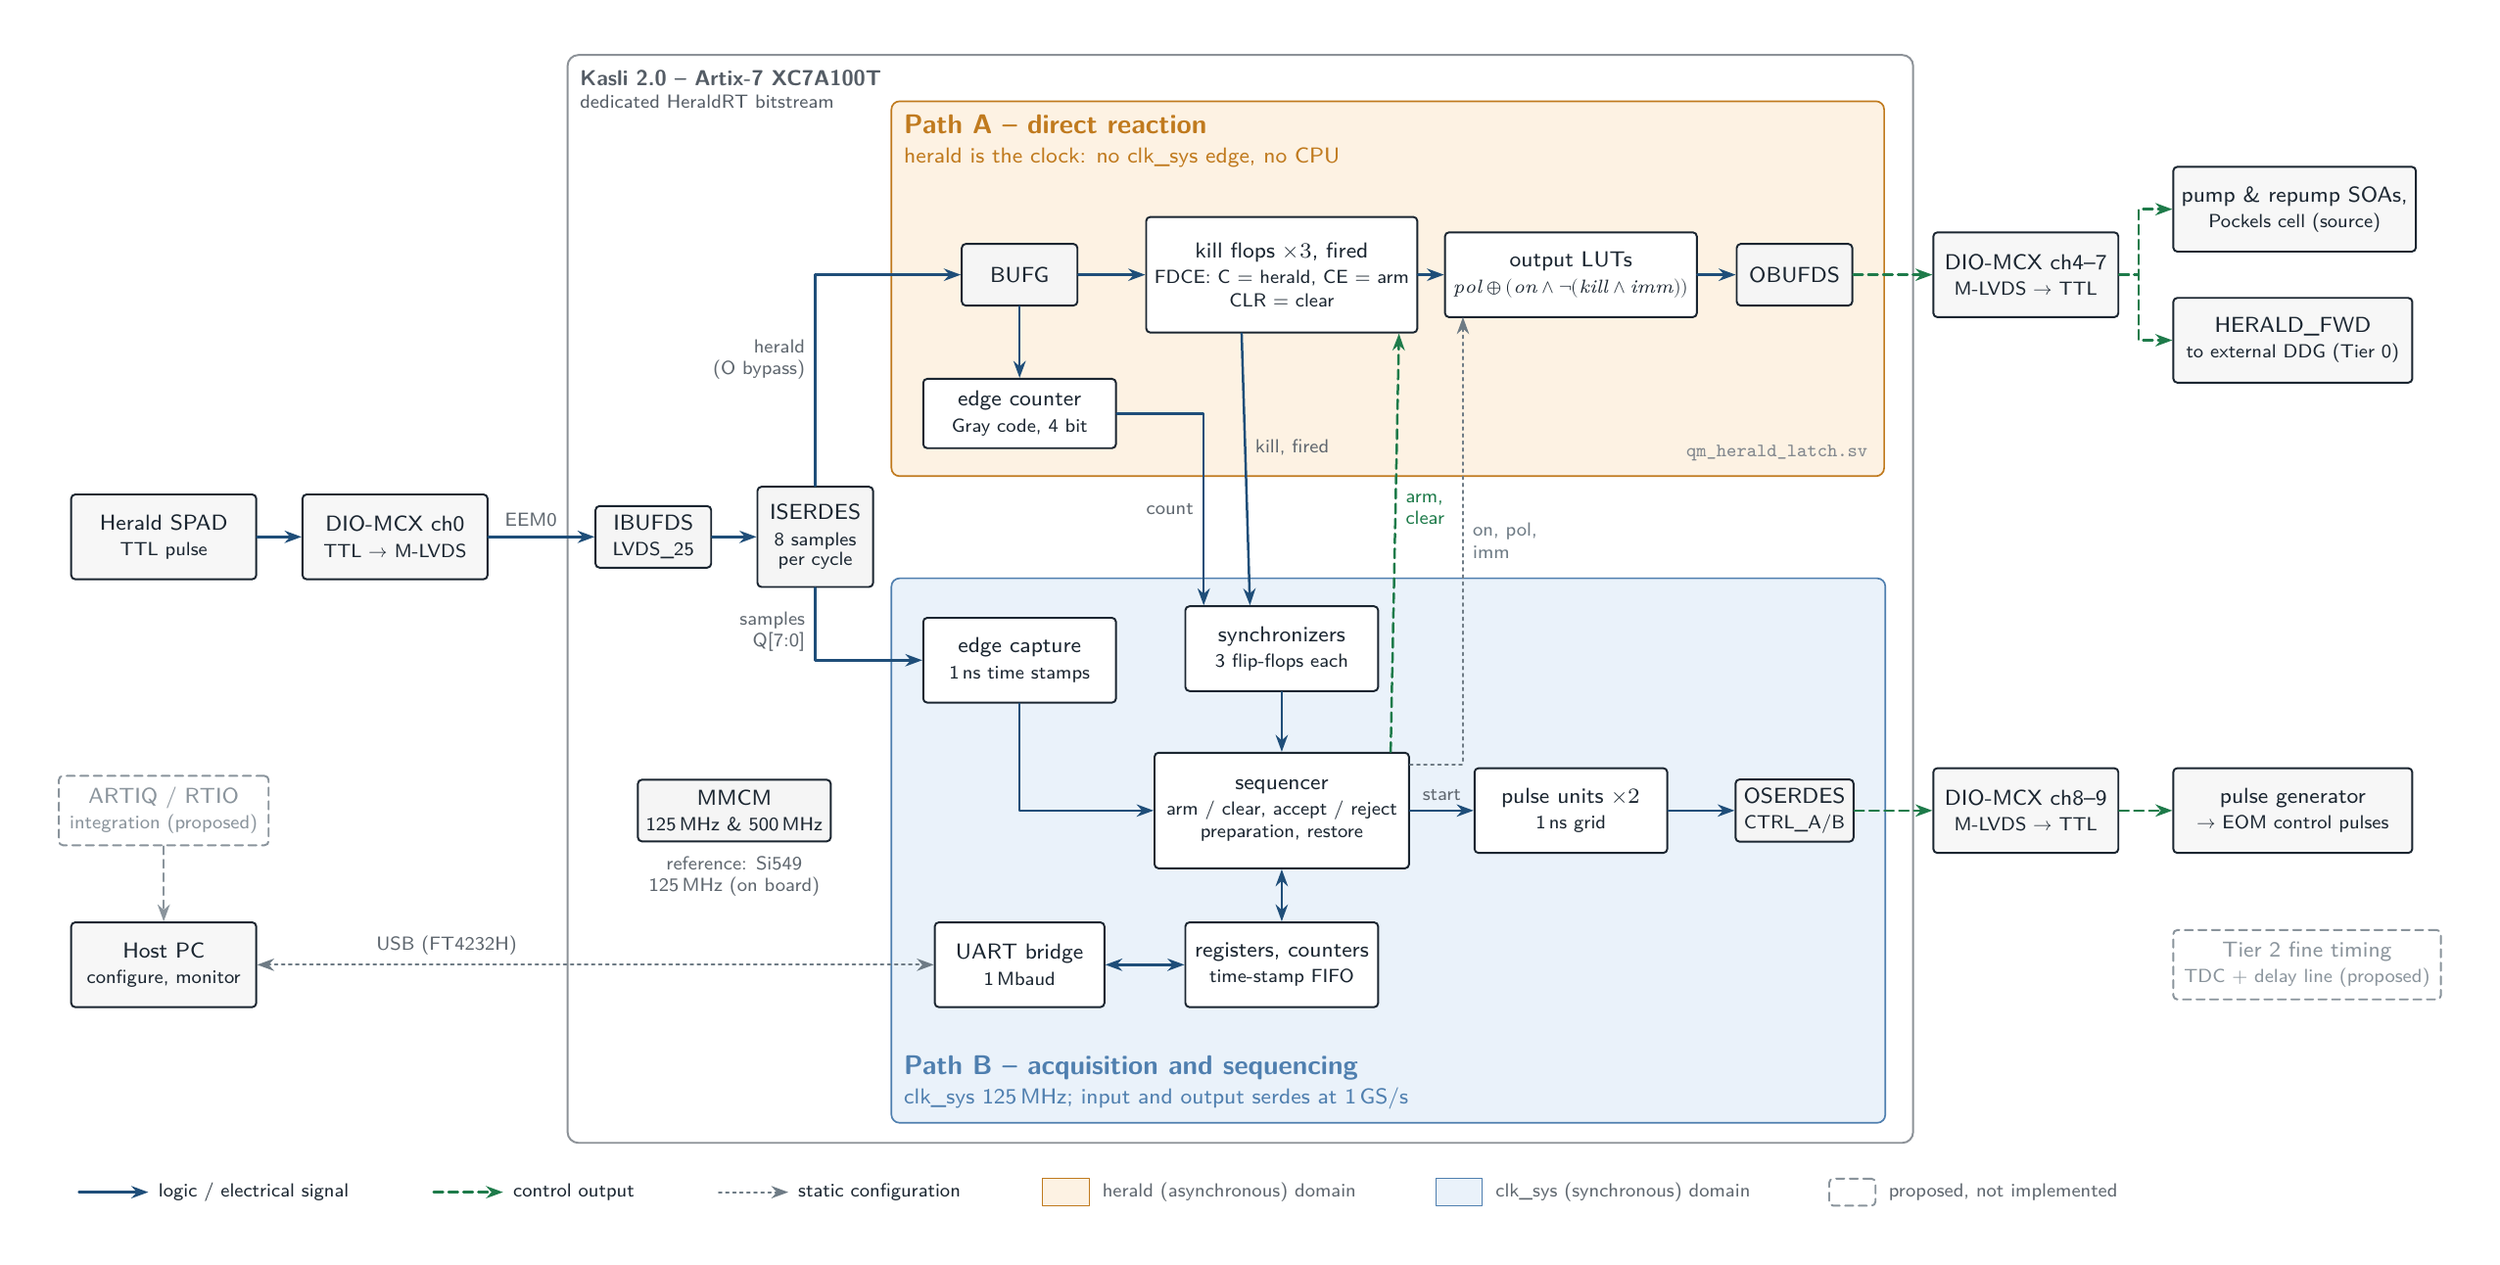
\begin{tikzpicture}[white page]
  \tikzset{
    rtl/.style  = {smallblock, minimum width = 25mm, minimum height = 11mm},
    wide/.style = {rtl, minimum width = 33mm, minimum height = 15mm},
    prim/.style = {smallblock, minimum width = 15mm, minimum height = 8mm, fill = black!4},
    ext/.style  = {smallblock, minimum width = 24mm, minimum height = 11mm, fill = black!3},
    file/.style = {font = \ttfamily\scriptsize, text = ink!55},
    cfg/.style  = {draw = host, line width = 0.7pt, dash pattern = on 1pt off 1.6pt, ->},
  }

  % ============================================================ input side
  \node[ext] (spad)  at (-2.7, 0) {Herald SPAD\\{\scriptsize TTL pulse}};
  \node[ext] (dioin) at (0.3, 0)  {DIO-MCX ch0\\{\scriptsize TTL $\rightarrow$ M-LVDS}};
  \node[prim] (ibuf) at (3.65, 0) {IBUFDS\\{\scriptsize LVDS\_25}};
  \node[prim, minimum height = 13mm] (iser) at (5.75, 0) {ISERDES\\{\scriptsize 8 samples}\\[-2pt]{\scriptsize per cycle}};
  \draw[elec] (spad) -- (dioin);
  \draw[elec] (dioin) -- node[above, tag, pos = 0.4] {EEM0} (ibuf);
  \draw[elec] (ibuf) -- (iser);

  % ============================================================ Path A (herald domain)
  \node[prim] (bufg) at (8.4, 3.4) {BUFG};
  \node[wide] (kill) at (11.8, 3.4)
       {kill flops $\times 3$, fired\\{\scriptsize FDCE: C = herald, CE = arm}\\[-1pt]{\scriptsize CLR = clear}};
  \node[rtl, minimum width = 31mm] (olut) at (15.55, 3.4)
       {output LUTs\\{\scriptsize $\mathit{pol} \oplus (\mathit{on} \wedge \neg(\mathit{kill} \wedge \mathit{imm}))$}};
  \node[prim] (obuf) at (18.45, 3.4) {OBUFDS};
  \node[rtl, minimum height = 9mm] (gray) at (8.4, 1.6) {edge counter\\{\scriptsize Gray code, 4 bit}};

  \draw[elec] (iser.north) |- node[pos = 0.3, left, tag, align = right] {herald\\(O bypass)} (bufg.west);
  \draw[elec] (bufg) -- (kill);
  \draw[elec] (bufg) -- (gray);
  \draw[elec, line width = 1.25pt] (kill) -- (olut);
  \draw[elec, line width = 1.25pt] (olut) -- (obuf);

  \coordinate (Atop) at (8.0, 5.3);
  \begin{pgfonlayer}{domains}
    \node[domain async, fit = (bufg) (kill) (olut) (obuf) (gray) (Atop), inner ysep = 3.5mm,
          inner xsep = 4mm] (pathA) {};
  \end{pgfonlayer}
  \node[domain label, font = \normalsize\bfseries, anchor = north west, text = asyncline]
       at ($(pathA.north west) + (0.05, -0.06)$)
       {Path A -- direct reaction\\[-1pt]{\footnotesize\mdseries herald is the clock: no clk\_sys edge, no CPU}};
  \node[file, anchor = south east] at ($(pathA.south east) + (-0.1, 0.08)$) {qm\_herald\_latch.sv};

  % ============================================================ Path B (clk_sys domain)
  \node[rtl]  (cap)   at (8.4, -1.6)  {edge capture\\{\scriptsize \SI{1}{ns} time stamps}};
  \node[rtl]  (sync)  at (11.8, -1.45) {synchronizers\\{\scriptsize 3 flip-flops each}};
  \node[wide] (seq)   at (11.8, -3.55)
       {sequencer\\{\scriptsize arm / clear, accept / reject}\\[-1pt]{\scriptsize preparation, restore}};
  \node[rtl]  (pulse) at (15.55, -3.55) {pulse units $\times 2$\\{\scriptsize \SI{1}{ns} grid}};
  \node[prim] (oser)  at (18.45, -3.55) {OSERDES\\{\scriptsize CTRL\_A/B}};
  \node[rtl]  (regs)  at (11.8, -5.55) {registers, counters\\{\scriptsize time-stamp FIFO}};
  \node[rtl, minimum width = 22mm] (uart) at (8.4, -5.55) {UART bridge\\{\scriptsize \SI{1}{Mbaud}}};

  \draw[elec] (iser.south) |- node[pos = 0.3, left, tag, align = right] {samples\\Q[7:0]} (cap.west);
  \draw[elec] (cap.south) |- (seq.west);
  \draw[elec] (sync) -- (seq);
  \draw[elec] (seq) -- node[above, tag] {start} (pulse);
  \draw[elec] (pulse) -- (oser);
  \draw[elec, <->] (seq) -- (regs);
  \draw[elec, <->] (regs) -- (uart);

  \coordinate (Bbot) at (8.0, -7.25);
  \begin{pgfonlayer}{domains}
    \node[domain sync, fit = (cap) (sync) (seq) (pulse) (oser) (regs) (uart) (Bbot), inner ysep = 3.5mm,
          inner xsep = 4mm] (pathB) {};
  \end{pgfonlayer}
  \node[domain label, font = \normalsize\bfseries, anchor = south west, text = syncline]
       at ($(pathB.south west) + (0.05, 0.06)$)
       {Path B -- acquisition and sequencing\\[-1pt]{\footnotesize\mdseries clk\_sys \SI{125}{MHz}; input and output serdes at \SI{1}{GS/s}}};

  % ============================================================ domain crossings
  \draw[elec] ($(kill.south west) + (1.25, 0)$) -- node[right, tag, pos = 0.42] {kill, fired}
              ($(sync.north west) + (0.85, 0)$);
  \draw[elec] (gray.east) -| node[pos = 0.75, left, tag] {count} ($(sync.north west) + (0.25, 0)$);
  \draw[ctrl] ($(seq.north east) + (-0.25, 0)$) -- node[right, tag, text = ctrl, pos = 0.58, align = left]
              {arm,\\clear} ($(kill.south east) + (-0.25, 0)$);
  \draw[cfg]  (seq.east |- 0, -2.95) -- (14.15, -2.95) -- node[right, tag, text = host, pos = 0.5, align = left]
              {on, pol,\\imm} (14.15, 2.85);

  % ============================================================ clocking
  \node[prim, minimum width = 24mm] (mmcm) at (4.7, -3.55) {MMCM\\{\scriptsize \SI{125}{MHz} \& \SI{500}{MHz}}};
  \node[tag, below = 0.6mm of mmcm, align = center] {reference: Si549\\\SI{125}{MHz} (on board)};

  % ============================================================ FPGA outline
  \coordinate (Ftop) at (3.0, 6.0);
  \begin{pgfonlayer}{board}
    \node[board, fit = (ibuf) (iser) (pathA) (pathB) (mmcm) (Ftop), inner xsep = 3.5mm, inner ysep = 2.5mm,
          draw = ink!50] (fpga) {};
  \end{pgfonlayer}
  \node[domain label, anchor = north west, text = ink!75] at ($(fpga.north west) + (0.05, -0.08)$)
       {Kasli 2.0 -- Artix-7 XC7A100T\\[-1pt]{\scriptsize\mdseries dedicated HeraldRT bitstream}};

  % ============================================================ outputs
  \node[ext] (dioA) at (21.45, 3.4)   {DIO-MCX ch4--7\\{\scriptsize M-LVDS $\rightarrow$ TTL}};
  \node[ext] (dioB) at (21.45, -3.55) {DIO-MCX ch8--9\\{\scriptsize M-LVDS $\rightarrow$ TTL}};
  \draw[ctrl] (obuf) -- (dioA);
  \draw[ctrl] (oser) -- (dioB);

  \node[ext, minimum width = 31mm, anchor = west] (eqA) at (23.35, 4.25) {pump \& repump SOAs,\\{\scriptsize Pockels cell (source)}};
  \node[ext, minimum width = 31mm, anchor = west] (fwd) at (23.35, 2.55) {HERALD\_FWD\\{\scriptsize to external DDG (Tier 0)}};
  \node[ext, minimum width = 31mm, anchor = west] (eqB) at (23.35, -3.55) {pulse generator\\{\scriptsize $\rightarrow$ EOM control pulses}};
  \draw[ctrl] (dioA.east) -- ++(0.25, 0) |- (eqA.west);
  \draw[ctrl] (dioA.east) -- ++(0.25, 0) |- (fwd.west);
  \draw[ctrl] (dioB) -- (eqB);
  \node[proposedblock, font = \footnotesize, minimum width = 31mm, anchor = west] (tier2) at (23.35, -5.55)
       {Tier 2 fine timing\\{\scriptsize TDC + delay line (proposed)}};

  % ============================================================ host
  \node[ext] (hostpc) at (-2.7, -5.55) {Host PC\\{\scriptsize configure, monitor}};
  \draw[hostlink] (hostpc) -- node[above, tag, pos = 0.28] {USB (FT4232H)} (uart);
  \node[proposedblock, font = \footnotesize, minimum width = 24mm] (artiq) at (-2.7, -3.55)
       {ARTIQ / RTIO\\{\scriptsize integration (proposed)}};
  \draw[draw = proposed, line width = 0.7pt, dash pattern = on 3pt off 2pt, ->] (artiq) -- (hostpc);

  % ============================================================ legend
  \begin{scope}[shift = {(-3.8, -8.5)}]
    \draw[elec] (0, 0) -- (0.9, 0) node[right, tag, text = ink] {logic / electrical signal};
    \draw[ctrl] (4.6, 0) -- (5.5, 0) node[right, tag, text = ink] {control output};
    \draw[cfg]  (8.3, 0) -- (9.2, 0) node[right, tag, text = ink] {static configuration};
    \node[draw = asyncline, fill = asyncfill, minimum width = 6mm, minimum height = 3.5mm] at (12.8, 0) {};
    \node[right, tag] at (13.15, 0) {herald (asynchronous) domain};
    \node[draw = syncline, fill = syncfill, minimum width = 6mm, minimum height = 3.5mm] at (17.9, 0) {};
    \node[right, tag] at (18.25, 0) {clk\_sys (synchronous) domain};
    \node[proposedblock, minimum width = 6mm, minimum height = 3.5mm, inner sep = 0pt] at (23.0, 0) {};
    \node[right, tag] at (23.35, 0) {proposed, not implemented};
  \end{scope}
\end{tikzpicture}
\end{document}
